\documentclass[12pt,a4paper]{article}
\usepackage[utf8]{inputenc}
\usepackage[T1]{fontenc}
\usepackage{babel}
\babelprovide[import,main]{spanish}
\usepackage{lmodern,microtype}
\usepackage[margin=2.5cm,headheight=15pt]{geometry}
\usepackage{booktabs,longtable,array,enumitem,xcolor,titlesec,fancyhdr,lastpage}
\usepackage{tikz,needspace}
\usetikzlibrary{arrows.meta,positioning}
\PassOptionsToPackage{obeyspaces}{url}
\usepackage{hyperref}
\definecolor{sectionblue}{RGB}{31,78,121}
\hypersetup{colorlinks=true,linkcolor=sectionblue,urlcolor=sectionblue,citecolor=sectionblue,
 pdftitle={Reimplementación compatible de OpenStack Placement: Etapa 2},pdfauthor={Paolo Castañon Barrera}}
\titleformat{\section}{\Large\bfseries\color{sectionblue}}{\thesection}{0.8em}{}
\titleformat{\subsection}{\normalsize\bfseries}{\thesubsection}{0.8em}{}
\titlespacing*{\section}{0pt}{16pt}{9pt}
\titlespacing*{\subsection}{0pt}{12pt}{6pt}
\setlength{\parindent}{0pt}
\setlength{\parskip}{6pt}
\setcounter{tocdepth}{2}
\emergencystretch=2em
\raggedbottom
\clubpenalty=10000
\widowpenalty=10000
\setlist{nosep,topsep=5pt,leftmargin=*}
\renewcommand{\tablename}{Cuadro}
\addto\captionsspanish{\renewcommand{\tablename}{Cuadro}}
\pagestyle{fancy}
\fancyhf{}
\fancyhead[L]{\small Trabajo de Título -- Etapa 2}
\fancyhead[R]{\small INFO-1197}
\fancyfoot[C]{\small\thepage\ de \pageref{LastPage}}
\renewcommand{\headrulewidth}{0.4pt}
\renewcommand{\footrulewidth}{0pt}
\newcommand{\code}[1]{{\small\expandafter\nolinkurl\expandafter{\detokenize{#1}}}}
\newcommand{\reporttable}[4]{\begingroup\small\setlength{\LTpre}{8pt}\setlength{\LTpost}{8pt}\setlength{\tabcolsep}{4pt}\renewcommand{\arraystretch}{1.15}
\begin{longtable}{#2}\caption{#1}\\\toprule #3\\\midrule\endfirsthead
\toprule #3\\\midrule\endhead\bottomrule\endfoot #4\end{longtable}\endgroup}
\newcommand{\reportcover}{
\hypersetup{pageanchor=false}
\begin{titlepage}\centering
\vspace*{0.3cm}
{\Large Universidad Católica de Temuco\par}
\vspace{0.2cm}{\large Ingeniería Civil en Informática\par}
\vspace{2cm}
{\LARGE\bfseries Reimplementación compatible de\\OpenStack Placement\\en un lenguaje compilado\par}
\vspace{0.65cm}
{\large\bfseries Etapa 2: análisis, diseño y línea base\par}
\vspace{1.8cm}
\begin{tabular}{rl}
\textbf{Estudiante:}&Paolo Castañon Barrera\\[0.35cm]
\textbf{Profesor guía:}&Alejandro Mellado Gatica\\[0.35cm]
\textbf{Curso:}&Trabajo de Título (INFO-1197)\\[0.35cm]
\textbf{Fecha:}&2 de octubre de 2026
\end{tabular}
\vfill Temuco, Chile
\end{titlepage}
\pagenumbering{arabic}\hypersetup{pageanchor=true}\tableofcontents\newpage}
\begin{document}
\reportcover

\section{Introducción}
OpenStack Placement registra capacidad y uso de recursos para apoyar la selección de destinos de cómputo. Nova consulta este servicio durante la planificación y mantiene asignaciones asociadas a cada instancia. Su API HTTP ofrece un límite de integración adecuado para estudiar una reimplementación en un lenguaje compilado \cite{placementapi,nova}.

Este informe corresponde al trabajo de Paolo Castañon Barrera y concentra el análisis en Placement. Se conserva la organización del informe de Etapa 1: problema, objetivos, requerimientos, planificación y conclusiones. La Etapa 2 desarrolla esos apartados con arquitectura, contrato de API, modelo de datos, decisiones de diseño y evidencia del laboratorio.

La propuesta utiliza Go y evalúa dos dimensiones: compatibilidad funcional y comportamiento bajo carga. La mejora de rendimiento es una hipótesis que debe medirse. En esta etapa se verificó el servicio original; la implementación Go y los benchmarks comparativos corresponden a las etapas siguientes.

El entorno es compartido con el proyecto de Glance, pero el objeto de estudio de este documento es Placement. Los resultados comunes de infraestructura se identifican como tales y no se presentan como mediciones exclusivas del módulo ni como atribución individual de la ejecución.

\section{Definición del problema}
\subsection{Contexto}
El despliegue de una instancia requiere coordinar Nova, Keystone, Neutron, Glance y Placement. En el flujo de planificación, Placement entrega candidatos que satisfacen recursos y restricciones; Nova decide el destino y registra el consumo. El servicio combina semántica HTTP, negociación de microversiones y reglas de consistencia persistente \cite{placementapi,nova}.

La línea base se obtuvo en una instalación DevStack de un nodo. Esta configuración permite observar llamadas reales y repetir escenarios controlados. No representa un despliegue de producción ni una evaluación de escalado multinodo.

\subsection{Problema identificado}
Cambiar el lenguaje de implementación puede alterar códigos HTTP, formatos JSON, errores, filtrado de candidatos o control de concurrencia. Un servidor que responde a rutas conocidas no demuestra por sí solo que Nova pueda utilizarlo. La dificultad técnica es conservar el contrato observable del subconjunto necesario y medir sus costos con una comparación repetible.

La pregunta de investigación es: \textit{¿es posible reimplementar el alcance seleccionado de Placement en Go, conservando la integración con Nova, y qué diferencias de latencia, throughput y uso de recursos se observan frente al servicio original?}

\subsection{Relevancia e impacto}
La contribución esperada es una especificación verificable y una implementación experimental integrada. El trabajo puede identificar costos de procesamiento HTTP, acceso a datos y búsqueda de candidatos; también puede mostrar regresiones o límites de compatibilidad. La validez del resultado depende de reportar ambos tipos de hallazgo.

\subsection{Partes interesadas y percepción del problema}
\reporttable{Partes interesadas del proyecto Placement.}{>{\raggedright\arraybackslash}>{\raggedright\arraybackslash}p{3.6cm}>{\raggedright\arraybackslash}p{11.4cm}}{\textbf{Parte interesada}&\textbf{Necesidad o interés}}{
Estudiante responsable&Paolo Castañon Barrera: delimitar, diseñar e implementar Placement y sustentar las conclusiones con pruebas.\\*
Profesor guía&Revisar coherencia entre problema, alcance, evidencia y resultados del trabajo de título.\\*
Consumidores de la API&Nova y clientes de OpenStack: conservar el contrato HTTP y la consistencia del estado.\\*
Equipo del laboratorio&Reconstruir el entorno común y aislar la sustitución de cada servicio.\\}

\subsection{Alcance y límites}
Se incluyen proveedores de recursos, inventarios, clases de recursos, traits, allocations y candidatos utilizados en el escenario de un nodo. El análisis contempla autenticación Keystone, persistencia y generaciones para resolver conflictos.

El servidor original anuncia microversiones 1.0 a 1.39. La propuesta inicial selecciona 1.0, 1.2, 1.6, 1.10, 1.28 y 1.36 según la operación; esto no equivale a implementar todas las microversiones intermedias ni toda la API. \texttt{\small POST}\,\code{/reshaper}, migraciones complejas de inventario y topologías no exigidas por las pruebas quedan fuera del alcance inicial.

Glance se mantiene como dependencia original al probar la sustitución de Placement. No se reimplementan Nova, Keystone, Neutron ni el sistema de virtualización. Tampoco se promete sustituir una base de datos existente sin un procedimiento de migración.

\Needspace{165pt}
\section{Objetivos}
\subsection{Objetivo general}
Diseñar, implementar y evaluar una reimplementación compatible del subconjunto seleccionado de OpenStack Placement en Go, integrada con Nova en un laboratorio reproducible, comparando su funcionamiento, rendimiento y uso de recursos con el servicio original.

\subsection{Objetivos específicos}
Los identificadores OE1--OE5 conservan la trazabilidad de la planificación común; su redacción aquí se aplica a Placement. El porcentaje del hito OE3 corresponde al proyecto conjunto y no se utiliza como medida de avance individual.
\begin{enumerate}[label=\textbf{OE\arabic*.}]
\item Analizar arquitectura, API, dependencias, datos e interacción Nova--Placement antes del 2 de octubre de 2026.
\item Disponer de un entorno reproducible y una línea base funcional del servicio original antes del 2 de octubre de 2026.
\item Implementar al menos el 50\% del alcance comprometido, con pruebas preliminares, antes del 30 de octubre de 2026.
\item Integrar y estabilizar el alcance de Placement con Nova antes del 20 de noviembre de 2026.
\item Comparar compatibilidad, latencia, throughput, CPU, memoria y errores, y presentar conclusiones antes del 4 de diciembre de 2026.
\end{enumerate}

\subsection{Verificación SMART}
\reporttable{Objetivos, indicadores y estado al cierre de Sprint 2.}{>{\raggedright\arraybackslash}>{\raggedright\arraybackslash}p{1cm}>{\raggedright\arraybackslash}p{8cm}>{\raggedright\arraybackslash}p{2.5cm}>{\raggedright\arraybackslash}p{2.8cm}}{\textbf{ID}&\textbf{Indicador y evidencia}&\textbf{Plazo}&\textbf{Estado}}{
OE1&Arquitectura y rutas del alcance documentadas; modelo auditado y tráfico Nova registrado.&02-10-2026&Cumplido en S2.\\*
OE2&Laboratorio instalado; smoke test y baseline ejecutados; instancia en ACTIVE y limpieza.&02-10-2026&Cumplido en S2.\\*
OE3&Al menos 50\% del alcance priorizado implementado y probado en Go.&30-10-2026&Planificado.\\*
OE4&Prueba de sustitución con Nova y casos críticos sin regresiones.&20-11-2026&Planificado.\\*
OE5&Dataset comparable, repeticiones y análisis de métricas y limitaciones.&04-12-2026&Planificado.\\}
La medición de OE1 se refiere al alcance documentado para Sprint 2. Los endpoints definidos pero aún no ejercitados quedan señalados para ampliar sus fixtures; no se infiere cobertura experimental total de la API.

\Needspace{220pt}
\subsection{Matriz de trazabilidad problema--objetivos}
\reporttable{Trazabilidad del problema Placement.}{>{\raggedright\arraybackslash}>{\raggedright\arraybackslash}p{4.4cm}>{\raggedright\arraybackslash}p{1.8cm}>{\raggedright\arraybackslash}p{8.7cm}}{\textbf{Aspecto del problema}&\textbf{Objetivo}&\textbf{Resultado verificable}}{
Contrato y versiones desconocidos&OE1&Inventario de métodos, rutas y microversiones; llamadas reales de Nova.\\*
Instalación y pruebas difíciles de repetir&OE2&Terraform, Ansible, versiones fijadas y scripts versionados.\\*
Consistencia y equivalencia del reemplazo&OE3/OE4&Transacciones, conflictos de generación y pruebas diferenciales/integradas.\\*
Hipótesis de eficiencia sin medir&OE5&Comparación controlada de latencia, throughput y recursos.\\}

\section{Análisis de requerimientos}
\subsection{Base técnica y arquitectura del servicio}
En el código desplegado se identifican entrada WSGI, middleware de autenticación, políticas, negociación de microversión, handlers HTTP, objetos de dominio y persistencia SQLAlchemy. Las generaciones de providers y consumers forman parte de las reglas de actualización. Estas capas se documentaron a partir del código del commit fijado y se contrastaron con API y tablas reales \cite{repo}.

\begin{figure}[ht]
\centering
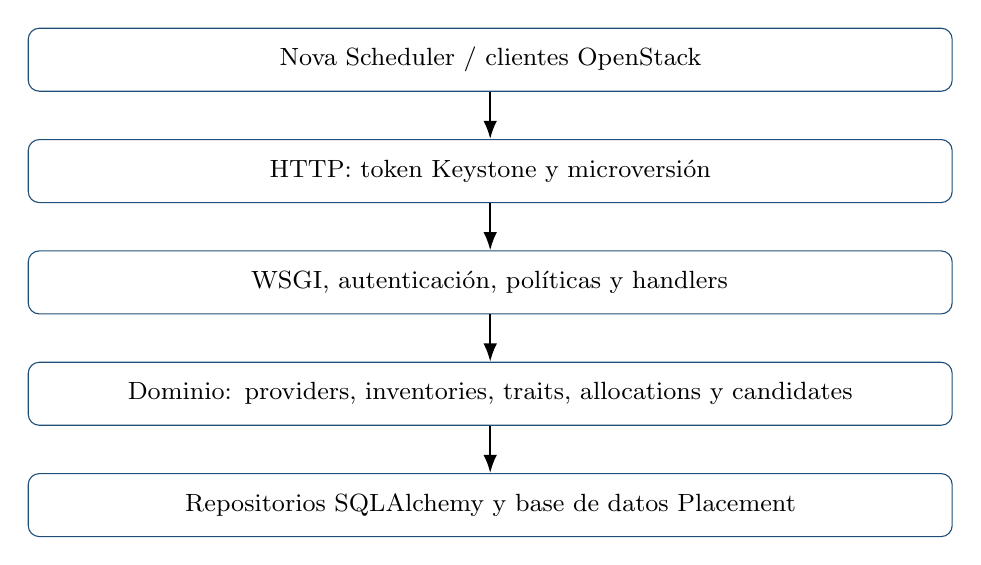
\begin{tikzpicture}[node distance=0.6cm,box/.style={draw=sectionblue,rounded corners,align=center,text width=11.5cm,minimum height=0.8cm,font=\small},arr/.style={-{Latex},thick}]
\node[box](nova){Nova Scheduler / clientes OpenStack};
\node[box,below=of nova](api){HTTP: token Keystone y microversión};
\node[box,below=of api](wsgi){WSGI, autenticación, políticas y handlers};
\node[box,below=of wsgi](domain){Dominio: providers, inventories, traits, allocations y candidates};
\node[box,below=of domain](db){Repositorios SQLAlchemy y base de datos Placement};
\draw[arr](nova)--(api);\draw[arr](api)--(wsgi);\draw[arr](wsgi)--(domain);\draw[arr](domain)--(db);
\end{tikzpicture}
\caption{Componentes del servicio original y límite HTTP de integración.}
\end{figure}

\subsection{Selección del servicio y del lenguaje}
Placement se selecciona por su función en la planificación de Nova y por disponer de un contrato HTTP que permite sustituir el proceso del servicio. La selección no implica que su comportamiento sea simple: generaciones, filtros y capacidad disponible deben conservarse.

Se propone Go por su biblioteca HTTP, compilación a binario y soporte de concurrencia. La valoración siguiente es una decisión de diseño del proyecto; no constituye un benchmark entre lenguajes.
\reporttable{Alternativas de lenguaje para la implementación Placement.}{>{\raggedright\arraybackslash}>{\raggedright\arraybackslash}p{4.3cm}>{\raggedright\arraybackslash}p{3.2cm}>{\raggedright\arraybackslash}p{3.2cm}>{\raggedright\arraybackslash}p{3.6cm}}{\textbf{Criterio}&\textbf{Go}&\textbf{Rust}&\textbf{C++}}{
Desarrollo HTTP&Biblioteca estándar y ecosistema adecuados.&Ecosistema adecuado; mayor curva inicial.&Requiere integrar bibliotecas.\\*
Memoria y concurrencia&Gestión automática; goroutines.&Control estricto de propiedad.&Mayor responsabilidad manual.\\*
Riesgo en el plazo&Moderado.&Mayor costo inicial estimado.&Mayor costo de integración estimado.\\*
Decisión&Seleccionado.&Alternativa.&No priorizado.\\}

\subsection{Entorno de despliegue: DevStack versus instalación manual}
DevStack automatiza un entorno de desarrollo y pruebas \cite{devstack}. Frente a una instalación manual, reduce la configuración inicial y permite concentrar el trabajo en compatibilidad. La instalación manual brinda control detallado, pero exige documentar más pasos y resolver dependencias por separado.

El laboratorio común utiliza Terraform con libvirt y Ansible. La VM \code{tt-openstack-lab} tiene Ubuntu 24.04.5, 4 vCPU, 8 GiB de RAM y disco de 55 GiB. Nova usa QEMU emulado. Se verificaron Keystone, Nova, Placement, Glance, Neutron, MySQL y RabbitMQ, y una segunda ejecución del aprovisionamiento terminó sin reinstalar DevStack.

\reporttable{Versiones registradas en la línea base.}{>{\raggedright\arraybackslash}>{\raggedright\arraybackslash}p{4cm}>{\raggedright\arraybackslash}p{11cm}}{\textbf{Componente}&\textbf{Versión o commit}}{
DevStack&\code{stable/2026.2}; \code{0fb9685c1bf22cd0b4d576d7a74f64195ad934fe}.\\*
Placement&\code{f4a89d3803cb23df22b8714569889ab39c918c34}.\\*
Nova&\code{247ea5d774305b688997f8df81c011b249eb793c}.\\*
Python / MySQL&3.12.3 / 8.0.46.\\*
OpenStackClient&10.3.0.\\}
La configuración y un parche de inicialización Geneve están versionados. Las dependencias secundarias no están fijadas para reproducción bit a bit. Al cierre del trabajo la VM quedó apagada por solicitud del usuario, conservando sus discos; este informe usa evidencia obtenida antes del apagado.

\subsection{Contrato API y microversiones}
La autenticación utiliza tokens Keystone. El contrato debe conservar entradas, respuestas, errores y headers relevantes para cada microversión. El cuadro distingue llamadas ejercitadas de operaciones todavía pendientes de captura.
\reporttable{Operaciones Placement priorizadas y cobertura de la línea base.}{>{\raggedright\arraybackslash}>{\raggedright\arraybackslash}p{6.8cm}>{\raggedright\arraybackslash}p{2.2cm}>{\raggedright\arraybackslash}p{6cm}}{\textbf{Método y ruta}&\textbf{Versión}&\textbf{Evidencia o estado}}{
\texttt{\small GET}\,\code{/}&Anunciada 1.0--1.39&Descubrimiento del servidor original.\\*
\texttt{\small GET/POST}\,\code{/resource_providers}&1.0&Listado y creación probados.\\*
\texttt{\small GET/DELETE}\,\code{/resource_providers/{uuid}}&1.0&Consulta, eliminación y 404 probados.\\*
\texttt{\small PUT}\,\code{/resource_providers/{uuid}}&1.0&Diseñado; fixture pendiente.\\*
\texttt{\small GET/PUT}\,\code{/resource_providers/{uuid}/inventories}&1.0&Consulta y reemplazo de inventarios probados.\\*
\texttt{\small GET}\,\code{/resource_classes}&1.2&Listado probado; consulta por nombre pendiente.\\*
\texttt{\small GET}\,\code{/resource_providers/{uuid}/traits}&1.6&Consulta probada; asociación y listado global pendientes.\\*
\texttt{\small GET}\,\code{/allocation_candidates}&1.10 / 1.36&Baseline y petición real de Nova, HTTP 200.\\*
\texttt{\small GET}\,\code{/allocations/{consumer}}&1.28&Petición real de Nova, HTTP 200.\\*
\texttt{\small PUT}\,\code{/allocations/{consumer}}&1.36&Reclamación real de Nova, HTTP 204.\\*
\texttt{\small DELETE}\,\code{/allocations/{consumer}}&1.0&Liberación real de Nova, HTTP 204.\\}
Para la implementación se requieren casos negativos de entradas inválidas, conflictos de generación y autorización. Un error 404 ya quedó registrado en la línea base, pero no se considera suficiente para aceptar todo el manejo de errores. Las clases personalizadas son condicionales; \code{reshaper} queda excluido inicialmente.

\subsection{Modelo de datos y consistencia}
La auditoría contrastó las tablas MySQL con los modelos SQLAlchemy del servicio fijado. Algunas relaciones son lógicas u ORM y no corresponden a una FK SQL declarada; el diseño evita asumir restricciones que la captura de tablas no demuestra.
\reporttable{Entidades centrales y restricciones relevantes.}{>{\raggedright\arraybackslash}>{\raggedright\arraybackslash}p{3.6cm}>{\raggedright\arraybackslash}p{6.2cm}>{\raggedright\arraybackslash}p{5.2cm}}{\textbf{Entidad}&\textbf{Datos centrales}&\textbf{Regla de diseño}}{
ResourceProvider&ID, UUID y nombre únicos; generación; relaciones padre/raíz.&Identidad estable y actualización con generación.\\*
Inventory&Provider, clase, total, reservado, límites, paso y ratio.&Unicidad provider/clase y validación de capacidad.\\*
ResourceClass / Trait&Identificador y nombre; asociaciones provider/trait.&Preservar clases y rasgos usados por Nova.\\*
Consumer&UUID, proyecto, usuario, generación y tipo.&Asociar consumo y controlar concurrencia.\\*
Allocation&Provider, consumer, clase y cantidad usada.&Operaciones atómicas y consistencia entre uso e inventario.\\}
Se decide usar un esquema propio en una base separada para Go y mantener compatibilidad por API. Esta decisión reduce acoplamiento con las migraciones Python, pero exige semillas y comparación del estado. Las transacciones deben comprobar capacidad y generaciones antes de confirmar allocations; las reglas concretas se validarán con fixtures diferenciales.

\subsection{Interacción Nova--Placement}
La traza real del boot confirma búsqueda de candidatos, consulta de allocations, reclamación y liberación. La consulta de Nova solicitó \code{DISK_GB:1,MEMORY_MB:512,VCPU:1} y restricciones \code{OWNER_NOVA,!COMPUTE_STATUS_DISABLED}. Scheduler seleccionó \code{tt-openstack-lab} y la instancia alcanzó ACTIVE.
\begin{enumerate}
\item Nova solicita candidatos y recibe HTTP 200 con microversión 1.36.
\item Consulta las allocations del consumer y recibe HTTP 200 con 1.28.
\item Registra la reclamación con PUT y recibe HTTP 204 con 1.36.
\item La eliminación de la instancia libera allocations mediante DELETE, HTTP 204 con 1.0.
\end{enumerate}
Los logs prueban método, ruta, resultado y microversión. No capturan el cuerpo completo de las solicitudes internas, por lo que aún se deben obtener fixtures específicos de esos cuerpos. El resultado ACTIVE valida la integración del original, no la de un reemplazo Go aún inexistente.

\Needspace{390pt}
\subsection{Requerimientos funcionales}
\reporttable{Requerimientos aplicables al módulo Placement.}{>{\raggedright\arraybackslash}>{\raggedright\arraybackslash}p{1.4cm}>{\raggedright\arraybackslash}p{8.8cm}>{\raggedright\arraybackslash}p{4.8cm}}{\textbf{ID}&\textbf{Requerimiento}&\textbf{Verificación prevista}}{
RF01&OpenStack de un nodo reproducible.&Instalación y smoke test; base validada en S2.\\*
RF02&Rutas y microversiones del alcance.&Suite de contrato y comparación de headers/JSON.\\*
RF03&Proveedores e inventarios compatibles.&CRUD, capacidad y conflictos.\\*
RF04&Traits y clases requeridos.&Consultas, asociaciones y filtros priorizados.\\*
RF05&Consulta y actualización de allocations.&Reclamación/liberación y generaciones.\\*
RF06&Candidatos compatibles con Nova.&Comparación semántica de candidatos y boot.\\*
RF07&Persistencia consistente.&Reinicio y transacciones concurrentes.\\*
RF08&Autenticación y políticas necesarias.&Casos autorizados, 401 y 403.\\*
RF09&Sustitución integrada con Nova.&Boot y eliminación usando Go.\\*
RF11 / RF12&Observabilidad y automatización.&Logs saneados, scripts y métricas repetibles.\\}
RF03--RF09 describen aceptación de la implementación futura. El análisis de Sprint 2 no equivale a tener estos requerimientos implementados en Go.

\subsection{Requerimientos no funcionales}
\reporttable{Atributos de calidad y criterios de verificación.}{>{\raggedright\arraybackslash}>{\raggedright\arraybackslash}p{1.5cm}>{\raggedright\arraybackslash}p{3.5cm}>{\raggedright\arraybackslash}p{10cm}}{\textbf{ID}&\textbf{Atributo}&\textbf{Criterio}}{
RNF01&Compatibilidad&Comparar status, tipos, campos, errores, headers estables y efectos persistidos.\\*
RNF02&Rendimiento&Latencia p50/p95/p99 y throughput con carga controlada.\\*
RNF03&Recursos&CPU y memoria del proceso en reposo y carga.\\*
RNF04&Fiabilidad&Repetir escenarios y registrar tasa de error.\\*
RNF05&Reproducibilidad&Versiones, configuración, comandos y dataset documentados.\\*
RNF06&Mantenibilidad&Capas separadas, pruebas y commits trazables.\\*
RNF07&Seguridad&Conservar autenticación y autorización; excluir secretos de fixtures.\\}

\subsection{Diseño objetivo y criterios de aceptación}
El ejecutable propuesto es \code{cmd/placement}. Los paquetes internos separan API, servicio, modelo y repositorio. Los handlers negocian versiones y validan HTTP; el servicio aplica reglas de negocio; el repositorio controla transacciones. Configuración, middleware Keystone y logging se mantienen como componentes reutilizables.

Se aceptará la sustitución cuando el original y Go superen los casos comprometidos, Nova cree y elimine una instancia utilizando Go, y las comparaciones diferenciales no muestren diferencias semánticas relevantes. UUID, timestamps, request IDs y orden no garantizado podrán normalizarse sin ocultar cambios de capacidad o asignación.

Las pruebas abarcarán unidad, contrato, comparación diferencial, integración y escenario completo. La evaluación posterior usará misma VM, versiones, estado inicial, carga, warm-up y número de repeticiones. No se impone una mejora de velocidad como criterio de aceptación ni se presentan benchmarks de esta etapa.

\subsection{Riesgos y mitigaciones}
\reporttable{Riesgos del desarrollo Placement.}{>{\raggedright\arraybackslash}>{\raggedright\arraybackslash}p{4.5cm}>{\raggedright\arraybackslash}p{1.5cm}>{\raggedright\arraybackslash}p{9cm}}{\textbf{Riesgo}&\textbf{Nivel}&\textbf{Mitigación}}{
Cobertura de microversiones mayor a la estimada&Alto&Priorizar llamadas reales de Nova y registrar exclusiones.\\*
Conflictos o sobreasignación&Alto&Pruebas de generación, capacidad y atomicidad antes de optimizar.\\*
Cambios en dependencias&Medio&Mantener SHA fijados y registrar paquetes secundarios.\\*
Benchmark sesgado por QEMU o estado&Medio&Comparar procesos bajo la misma configuración y reportar límites del laboratorio.\\*
Cuerpos Nova incompletos&Medio&Capturar fixtures saneados antes de aceptar la integración Go.\\*
Retroalimentación formal pendiente&Medio&Incorporar observaciones del profesor cuando estén disponibles.\\}

\section{Planificación y backlog}
\subsection{Épicas}
Se conservan las épicas del Excel vigente que son aplicables: E1 infraestructura y entorno; E2 análisis y compatibilidad; E3 reimplementación Placement; E4 integración OpenStack; E5 pruebas y benchmarking. E6 reimplementación Glance corresponde al informe independiente de ese módulo. La documentación y entrega acompañan estas actividades.

\Needspace{280pt}
\subsection{Backlog prioritario y estado del Sprint 2}
Los IDs del cuadro proceden del Excel vigente \cite{plan} y no del backlog preliminar del PDF de Etapa 1, cuya numeración fue refinada. Se conserva esa distinción para evitar asociar una evidencia al elemento equivocado.
\reporttable{Elementos de Sprint 2 relevantes para Placement.}{>{\raggedright\arraybackslash}>{\raggedright\arraybackslash}p{1cm}>{\raggedright\arraybackslash}p{8.1cm}>{\raggedright\arraybackslash}p{1.2cm}>{\raggedright\arraybackslash}p{4.5cm}}{\textbf{ID}&\textbf{Elemento}&\textbf{SP}&\textbf{Estado}}{
B01&Preparar VM de laboratorio (compartido).&3&Hecho: VM auditada.\\*
B02&Instalar DevStack de un nodo (compartido).&5&Hecho: servicios verificados.\\*
B03&Smoke tests del original (compartido).&5&Hecho: boot ACTIVE y limpieza.\\*
B04&Analizar arquitectura interna Placement.&5&Hecho: componentes y datos.\\*
B05&Documentar endpoints y microversiones.&5&Hecho: inventario y capturas.\\*
B06&Registrar interacción Nova--Placement.&5&Hecho: logs reales del flujo.\\}
Las tareas específicas de Placement suman 15 SP; las comunes, 13 SP. El Sprint 2 conjunto alcanzó 7/7 elementos y 33/33 SP al incluir B19 de Glance. Estas cifras describen la planificación compartida, no una estimación de productividad individual.

La evidencia está en \code{evidence/sprint2/placement/}, \code{evidence/sprint2/nova/} y \code{evidence/sprint2/tests/}. El registro de versiones es \code{infra/devstack/versions.lock}; la auditoría de tablas está en \code{evidence/sprint2/environment/database-schema-audit.txt}. Los documentos de contrato, modelo y flujo se encuentran en \code{docs/sprint2/}. La verificación \code{make sprint2-verify} aprobó los artefactos y evidencias requeridos.

\Needspace{240pt}
\subsection{Plan por sprints e hitos}
\reporttable{Hitos del módulo Placement.}{>{\raggedright\arraybackslash}>{\raggedright\arraybackslash}p{3.2cm}>{\raggedright\arraybackslash}p{2.4cm}>{\raggedright\arraybackslash}p{9.4cm}}{\textbf{Periodo}&\textbf{Hito}&\textbf{Resultado esperado}}{
Hasta 04-09&Etapa 1&Problema, objetivos y requerimientos iniciales.\\*
05-09 a 02-10&Etapa 2 / S2&Diseño, entorno, baseline y tráfico Nova registrados.\\*
03-10 a 30-10&Etapa 3 / S3&Al menos 50\% implementado; priorizar B07 providers/inventories, B08 traits/classes y B11 persistencia.\\*
31-10 a 20-11&Cierre / S4&Allocations, candidates, auth y sustitución integradas y estabilizadas.\\*
21-11 a 04-12&Evaluación / S5&Dataset comparativo, gráficos, conclusiones e informe final.\\}

\section{Conclusiones de la Etapa 2}
La etapa produjo una especificación de Placement respaldada por el servicio original: arquitectura y tablas contrastadas, alcance HTTP documentado, microversiones observadas y un flujo real de Nova que alcanzó ACTIVE y liberó recursos al eliminar la instancia.

OE1 y OE2 están cumplidos para el alcance de Sprint 2. La implementación Go, la sustitución y la evaluación de rendimiento siguen planificadas. Los fixtures pendientes y la captura de cuerpos internos deben resolverse a medida que se implemente cada contrato, conservando los límites explícitos.

El siguiente paso es desarrollar providers, inventories, traits/classes y persistencia, y compararlos con la línea base. El resultado de esta etapa habilita esa implementación sin anticipar conclusiones sobre eficiencia. La retroalimentación formal del profesor guía permanece pendiente de incorporación.

\Needspace{280pt}
\begingroup\small
\phantomsection\addcontentsline{toc}{section}{Referencias}
\begin{thebibliography}{9}
\bibitem{placementapi} OpenStack. \textit{Placement API Reference}. Referencia utilizada en el proyecto y en el informe de Etapa 1. \url{https://docs.openstack.org/api-ref/placement/}.
\bibitem{nova} OpenStack. \textit{Nova Scheduling}. \url{https://docs.openstack.org/nova/latest/reference/scheduling.html}.
\bibitem{devstack} OpenStack. \textit{DevStack Documentation}. \url{https://docs.openstack.org/devstack/latest/}.
\bibitem{repo} Proyecto \textit{modules-devstack-optimized}. Documentación y evidencias Sprint 2, capturadas el 2 de octubre de 2026. Directorios \code{docs/sprint2/}, \code{evidence/sprint2/} e \code{infra/}; registro de evidencia y matriz final de trazabilidad.
\bibitem{plan} \textit{Planificacion\_Trabajo\_Titulo\_OpenStack\_Placement\_Glance.xlsx} y copia de seguimiento Sprint 2. Hojas Objetivos\_SMART, Requerimientos, Backlog, Trazabilidad y Sprints. La copia original se mantiene inalterada.
\end{thebibliography}
\endgroup
\end{document}
